\chapter{Effektmoduler}\label{chap:DSP}

\section{Echo effektmodul}\label{sec:echo}
\note{ved ikke om det skal ligge her}
Et echo opstår når en lydbølge reflekteres tilbage på en overflade, sålede at den kan høres igen blot forsinket den tid, det tager for lyden at bevæge sig gennem luften.
Det vil sige at jo længere væk overfladen, som lyden reflekteres på, er fra udgangspunktet for lydkilden og hvor lyden høres, jo længere går der imellem den oprindelige lyd og echoet.
Et echo opstår som regel i et stort åbent område hvor der så er en eller flere store relativt ubrudte flader, såsom facaden på en stor bygning eller en bjergside.
Også i nogle tunneler der har den rigtige udformning kan der opnås en god echo effekt.
Ved et echo reflekteres lydbølgen oftest tilbage til kilden relativt få gange og gerne med en lidt stor forsinkelse.

\section{Implementering af echo effektmodul}
Vi ønsker at implementere en echo effekt der virker real time på microcontrolleren , således at der kan føres et lydsignal ind, og der med det samme kommer et modificeret lydsignal ud.
Dette gøres ved at gemme en dæmpet kopi af outputsignalet i en buffer og efter en valgt forsinkelse, i form af et bestemt antal samples, bliver dette gemte signal lagt til udgangsignalet og igen bliver en kopi af dette gemt,således at der dannes et feedbackloop som det ses på figur \ref{fig:echo_simulink}.

\begin{figure}[h]
	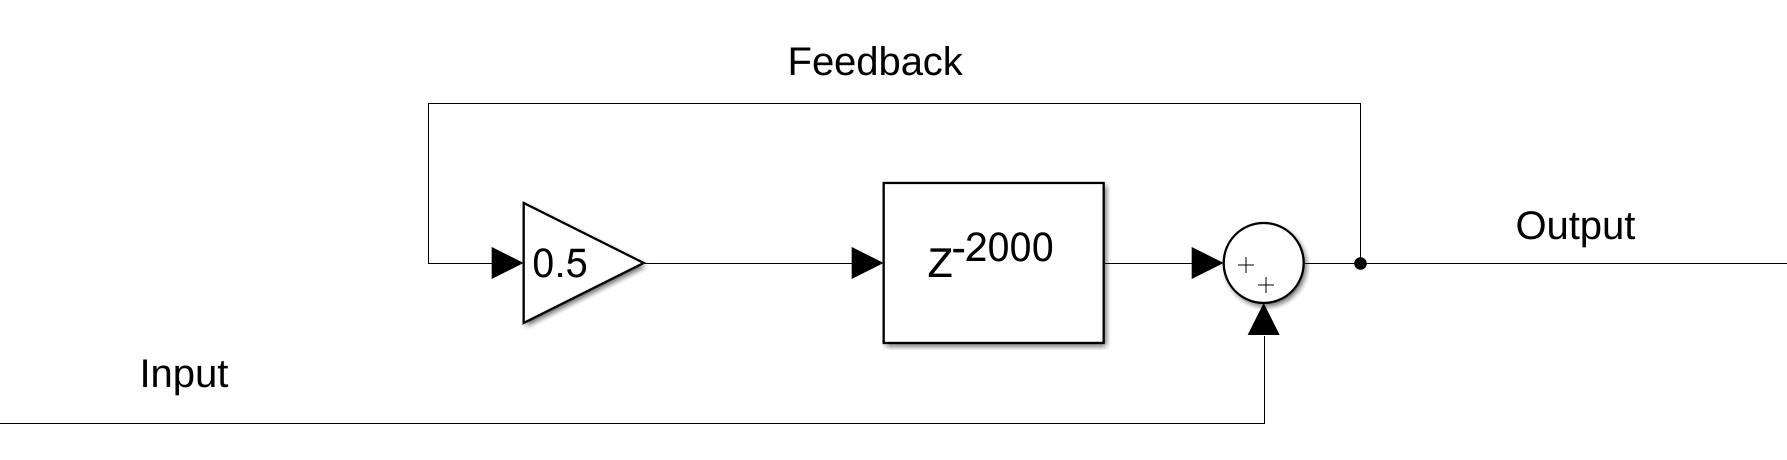
\includegraphics[width=0.8\linewidth]{./billeder/Echo_simulink.png}
	\caption{Simulink model af echo effekt.}
	\label{fig:echo_simulink}
\end{figure}

\section{Reverb effektmodul}\label{sec:reverb}

\husk{Sonny}{Har udkommenteret og forsøgt at uddybe afsnittet, kan stadig godt bruge feedback}
Reverb, rumklang, er resultatet af lydbølger som bliver reflekteret tilbage af %samtlige overflader med forskellige vinkler.\newline
%Rumklang er resultatet af lydbølger som bliver reflekteret af samtlige overflader i et rum, derved bygges der en masse reflektioner op hvis amplitude falder mod $0$ som de bliver absorberet af overfladerne i rummet.\newline
overfladerne i et givent lokale, dette påvirker lyden ud fra tre kriterier.\newline 
Et overfladerne kan bestå af forskellige materialer som afgør hvor stor en del af lydbølgen der reflekteres.\newline 
To afstanden mellem en given overflade, lydkilden og modtageren kan variere, dette giver reflektioner med forskellig forsinkelse samt forskellige amplituder da lydbølgen aftager i styrke jo længere den bevæger sig.\newline 
Tre overfladerne kan have forskellige vinkler som kan lede til at lydbølger reflekteres mellem en række overflader før de når modtageren, dette resultere i en kaskade af de effekter de andre to kriterier har.\newline
Der er to primære metoder for implementeringen af en digital reverb effekt convolution reverb og den algoritmisk reverb.
\subsection{Convolution reverb}
Reverberation, rumklang, er en tidsinvariant effekt, hvilket betyder at det ikke har nogen betydning, hvornår en tone bliver spillet, det vil ultimativt resultere i præcis den samme reverberation. \newline
Tidsinvariante systemer kan karakteriseres ved deres impulsrespons.
Et convolution reverb virker ved at lave en matematisk foldning af det ønskede %rummets 
impulsrespons og det lydsignal der skal tilføres en rumklang.\newline 
% sættes på indgange til reverben.\newline

%Dette skaber en realistisk rumklangseffekt, fordi impulsen i dette tilfælde vil være en lyd som holder samme energiniveau ved alle frekvenser.
En realistisk rumklangeffekt kan opnås ved at optage og anvende impulsresponsen fra et rum med den ønskede rumklang.
Dette gøres ved at producere en lyd impuls, et kort brag, eksempelvis ved at springe en ballon, og så optage den resulterende lyd. 
%Efter impulsen bliver spillet vil den blive reflekteret rundt i rummet.
%Nogle af reflektionerne møder mikrofonen med det samme mens andre bliver ført rundt i rummet og amplituden af signalerne går mod $0$ pga. overfladerne af objekterne i rummet absorbere energien fra dem.\newline
%Multiplikering af hver punkt af impulsresponset med amplituden af samplet giver så rummets respons til den sample.
Ved at multiplicere hvert punkt af impulsresponset med amplituden af en sample fås så rummets respons til den sample.
\husk{Sonny}{Nedenstående udkommenterede linje kunne godt tåle noget præcision}
%Dette gøres for hver sample af inputtet og giver overlappende responser som så adderes og resulterer i rumklang.
%En ulempe ved convolution reverbs er, at der skal mange beregninger til for at få resultatet.
De primære ulemper ved convolution reverb metoden er at der skal mange beregninger til for at få resultatet og at der skal anvendes en del hukommelse til at gemme impulsresponset fra rummet med en ønskede klang.
\husk{Sonny}{Frekvens/FFT?}
Da hver sample individuelt skal multipliceres med hver sample af impulsresponset og adderes til outputtet med den passende forsinkelse i tid, kan antallet af beregninger findes ved $N \cdot M$, hvor $N$ er antallet af samples impulsresponset fylder, altså samplings frekvensen multipliceret med længden af impulsresponset, og $M$ er samplings frekvensen.
Har man eksempelvis bruger et impulsrespons på $1$ sekund optaget ved $44.1\si{kHz}$ til at tilføje en rumklang til et stykke lyd der også bliver samplet ved $44.1\si{kHz}$, får man at det er nødvendigt med $1944810000$ multiplikations og additions  operationer i sekundet, altså lige knap $2$ milliarder operationer i sekundet. 
%Hvis der haves $N$ samples og impulsresponset er $M$ samples lang skal der udføres $N+M$ multiplikationer og additioner.
%F.eks. hvis der haves et impulsrespons på 1 sekund og der samples med $44.1\si{kHz}$, skal der udføres næsten 2 milliarder multiplikationer og additioner i sekundet.
%Antallet af multiplikationer og additioner kan dog reduceres drastisk ved at arbejde i frekvensdomænet i stedet for, da foldning i frekvensdomænet er multiplikation.

Fordelen ved convolution reverbs er at ethvert rum i verden kan imiteres, hvis impulsresponset for det valgte rum haves.\newline
Derudover kan man opfinde rum ved at syntetisere et impulsrespons.

\subsection{Algoritmisk reverb}
En algoritmisk reverb virker ved at bruge flere forskellige delays med tilhørende gains der sænker signalets styrke og feedback loops til at opbygge en serie af ekkoer, som dør ud over tid.
Det er sammensætningen af de basale byggeblokke som giver karakteristikken på rummet der emuleres.\newline
Et eksempel på en simpel algoritmisk reverb effekt er all-pass filteret.
%insert billede af all-pass filter
\begin{figure}[h]
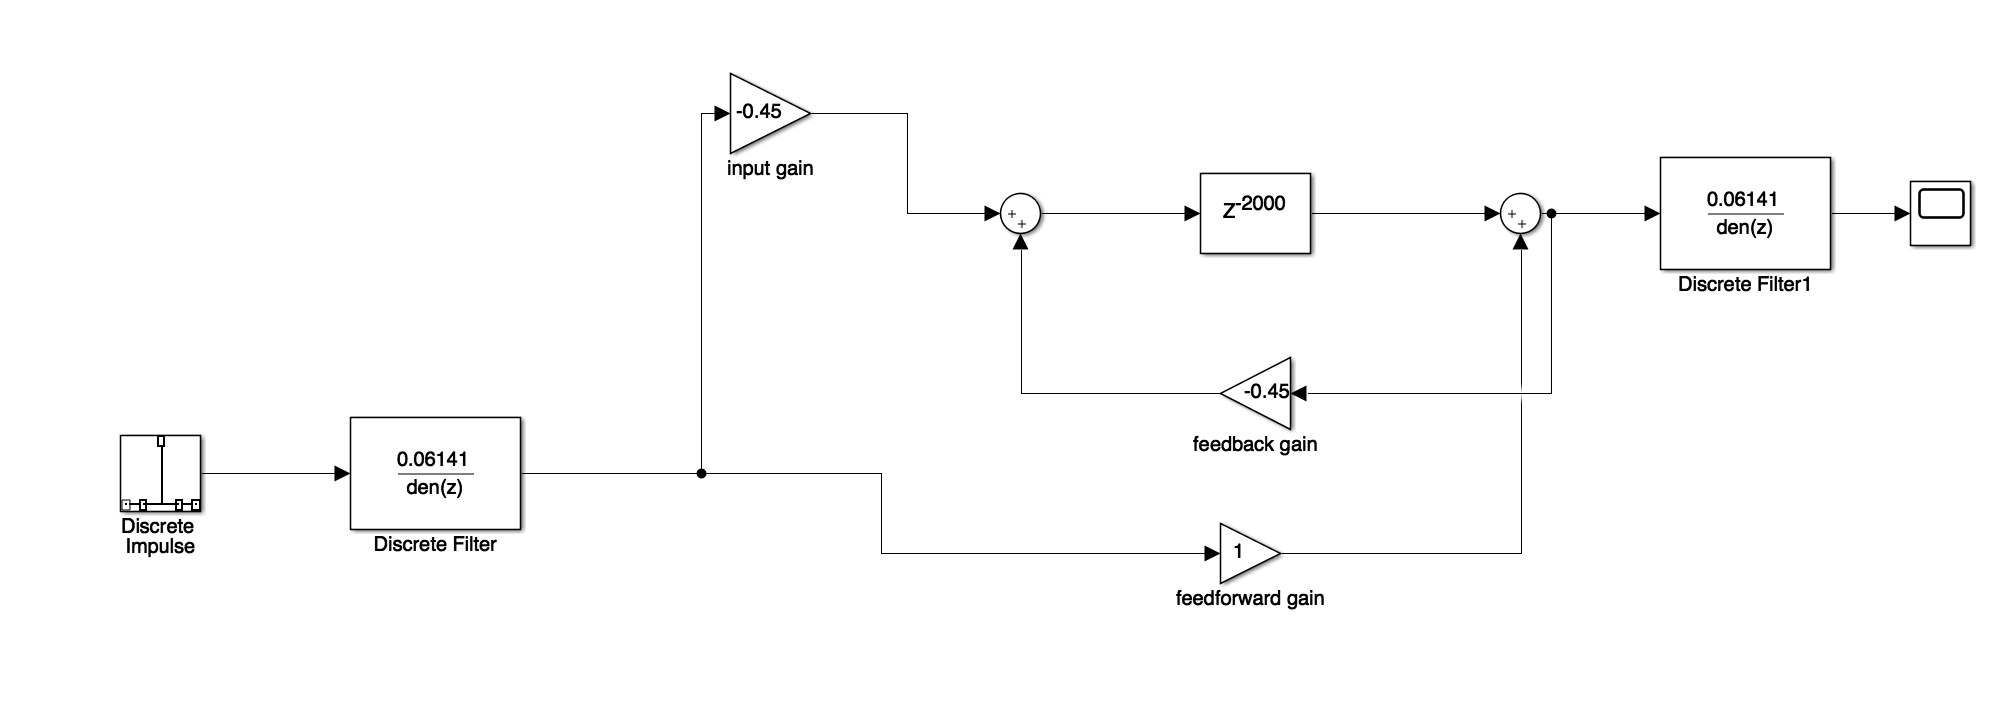
\includegraphics[width=0.8\linewidth]{./billeder/reverb-testopsaetning.png}
\caption{All-pass reverb filter i matlab.}
\label{fig:allPassMatLab}
\end{figure}
Her bliver en sample feeded forward til outputtet så lyden bliver spillet med det samme.
Derudover gemmes den i en reduceret og inverteret udgave. %smides samplet ind i en delay buffer.
%Rumklangen skabes så af samples fra delay bufferen, som fungerer som opbygningen af ekkoer og feedback loopet som agerer som absorptionen for at skabe aftagende ekkoer.
Rumklangen der skal tilføres til tiden fastsat af en delay tid kan så fremstilles af de gemte samples samt en brøkdel af outputtet.
Resultatet gemmes og bliver tillagt outputet til delay tiden og dermed opnås en række aftagende ekkoer.
Ulempen ved denne metode er at den skal serie kobles flere gange med forskellige delay tider for at opnå realistiske resultater.




\section{Implementering af reverb}
Gruppen valgte at implementere en algoritmisk reverb funktion da mikrochippen tilrådighed kun havde en meget begrænset mængde hukommelse.
Dette blev opnået ved at anvende en buffer til konstant at gemme reducerede samples af input og output som så kunne tilføjes outputtet til delay tiden.

Bufferen der blev valgt at implementere til dette er af en cyklisk natur, hvor der til hver samplingstid udlæses en værdi fra den af pointeren indikerede plads, pladsen nulstilles så og pointeren incrementeres så der til næste sample udlæses fra den næste plads i bufferen, herved opnås en buffer hvor der kan indsættes værdier der skal tilføres outputtet med en given forsinkelse angivet i antal samplingstider senere. 



\section{FIR filter}
Som et effektmodul blev der udviklet et FIR (finite impulse response) filter, hvilket vil sige at impulsresponset af filteret falder til nul efter et vist stykke tid.\newline
Et FIR filters overføringsfunktion er givet ved
\begin{equation}
H(z) = b_0 + b_1z^{-1} + \cdots + b_Kz^{-K}
\end{equation}
Hvori $b_i$ er filterets koefficienter.\cite[p.218]{Tan2013}\newline
Filteret og dets koefficienter bliver ved run-time beregnet efter brugeren inputter cutoff frekvensen. Filteret designes og det koefficienter bliver beregnet via frequency sampling metoden.
Grunden til frequency sampling valgtes som designmetode er, fordi algoritmen er baseret på invers diskret frekvens/tid fourier transformation (IDFT), hvilket kan beregnes effektivt via FFT.\newline
\section{Frequency Sampling}
Frequency sampling metoden virker ved at man lader $h(n)$ for $n = 0, 1, \cdots, N - 1$ approksimere filterets impulsrespons, hvor $N$ er antal koefficienter, hvilket for FIR filtre er deres koefficienter, og $H(k)$ for $k = 0, 1, \cdots, N - 1$ er de diskrete Fourier transformationskoefficienter.
\begin{figure}[!ht]
	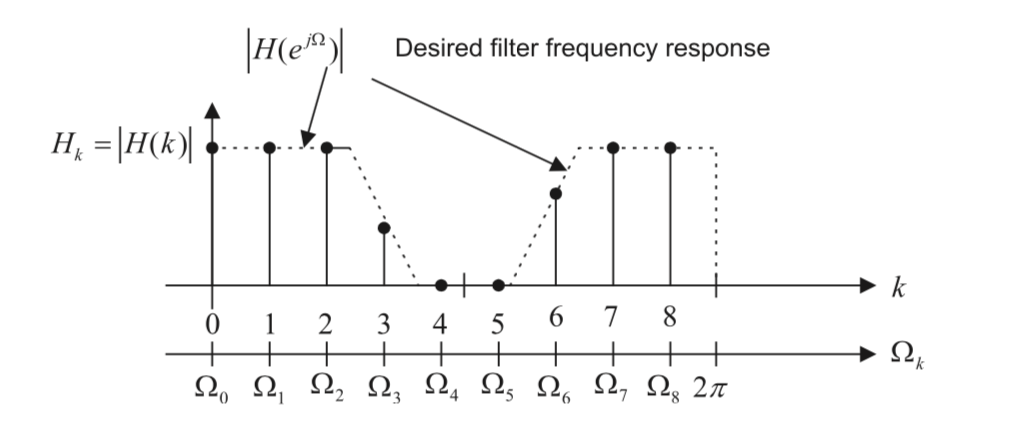
\includegraphics[width=\textwidth]{billeder/frequencysampling.png}
	\caption{Frekvenssampling af amplitudekarakteristik}
	\label{fig:frequencysampling}
\end{figure}
$H(k)$ findes ved at sample den ønskede amplitudekarakteristik i frekvensdomænet ved lige adskilte frekvenser som vist i figur \ref{fig:frequencysampling}.
FIR koefficienterne findes så ved
\begin{equation} \label{eq:fir_koefficienter}
b_n = h(n) = \frac{1}{2M + 1} \left\{H_0 + 2\displaystyle\sum_{k = 1}^{M}\, H_k\cos\left(\frac{2\pi k (n - M)}{2M + 1} \right) \right\} \quad \mathrm{for} \quad n = 0, 1, \cdots, M
\end{equation}
hvor $M = \frac{N - 1}{2}$
Resten af koefficienterne findes ved $h(n) = h(2M - n) \quad \mathrm{for} n = M + 1, \cdots, 2M$ ved brug af symmetri, når filteret antages at have lineær fase.


\subsection{Implementering af FIR filter}
Det digitale filter blev valgt at blive implementeret som et FIR filter, fordi FIR filtre giver mulighed for at have lineær negativ fase hvilket medfører konstant gruppeløbetid.\newline
Negativ lineær fase medfører konstant gruppeløbetid da gruppeløbetid er givet ved
\[
\tau = \frac{\mathrm{d}\varphi}{\mathrm{d}\omega}
\]
Konstant gruppeløbetid er en fordel at have i audio applikationer da en varierende gruppeløbetid kan komme til at lyde forkert.\newline
Modulet virker ved at det tager en cutoff frekvens som brugerinput og dernæst beregner normerede cutoff frekvens ved
\[ \Omega_c = 2\pi\frac{f_c}{f_s} \]
Hvor $f_c$ er cutoff frekvensen og $f_s$ er samplingsfrekvensen.
Dernæst beregnes en array af amplitudekarakteristikken $H_k$ for de normerede frekvenser fra $0$ til $\pi$ ved 
\[ \Omega_k = \frac{2\pi k}{(2M + 1)} \quad \mathrm{for} \quad k = 0, 1, \cdots, M \]
Når $H_k$ haves beregnes $M$ filterkoefficienter via. \ref{eq:fir_koefficienter} og resten findes ved symmetri.\newline
Filteret virker ved at en buffer fyldes med $x$ samples og dernæst bliver der foretaget en foldning for hver sampel i bufferen med hver filterkoefficient.

\section{Delkonklusion}
Echoeffekten blev implementeret via en delay buffer og et feedback loop således at inputtet bliver ført tilbage med en dæmpning på.\newline
Reverbeffekten blev implementeret som et all-pass filter, hvorved samples bliver ført ind i et dæmpningsled samt en delaybuffer samt at blive outputtet med det samme.
Filtereffekten blev implementeret som et FIR filter da disse giver mulighed for negativ lineær fase som medfører konstant gruppetid.
Der blev valgt frequency sampling som design metode, da den giver fine resultater og fordi algoritmen kræver relativt få beregninger, hvilket gør den godt egnet til real-time filter design.